\chapter{システム概要}
この章は2章で提案した手法を実現するために構築した双腕ロボットシステムを紹介する．基本的に先行研究で構築された料理ロボットシステムをそのまま利用した．

\section{ハードウェア}
	\subsection{双腕ロボット}\label{sec:robot}
	三菱重工製7自由度の汎用ロボットPA10-7Cを2台用いて，図\ref{fig:robot_system}のような双腕ロボットシステムを構築した．
	
	ロボットは,卓上での作業に従事し易いよう床面から約700[mm]の高さに設置した．
	各アームのベース座標系の原点は各アームの底の中央であり，各軸の向きはロボットから見た前方に$x$軸,ロボットから見て左側に$y$軸,鉛直上方に$z$軸となるように設定した．
	そして，今回の実験は両手同時に使う必要があるため，世界座標系が必要である．
	世界座標系は左ロボット(図\ref{fig:robot_system}に座標系がついているロボット)のベース座標系の原点として，各軸の向きは左ロボットのベース座標系と同じように設定した．
	次に，回転について，本論文はxyz軸周りのオイラー角度を使い，それぞれの回転角度は$\alpha,\beta,\gamma$として表す．プラス回転方向は図\ref{fig:robot_system}のように，回転軸を自分で指定し，逆時計回りの方向に設定した．
	また，各ロボットアームがお互いの動作を妨害せずに共同作業を可能とするために，両方のロボットアームが$Y$軸方向で804[mm]の間隔を設置した．
	最後に，両アームの手先には，(図\ref{fig:robot_force}、\ref{fig:robot_camera}、\ref{fig:robot_gripper})のように各種アタッチメントを装備した.
	\begin{figure}[h]
		\centering
		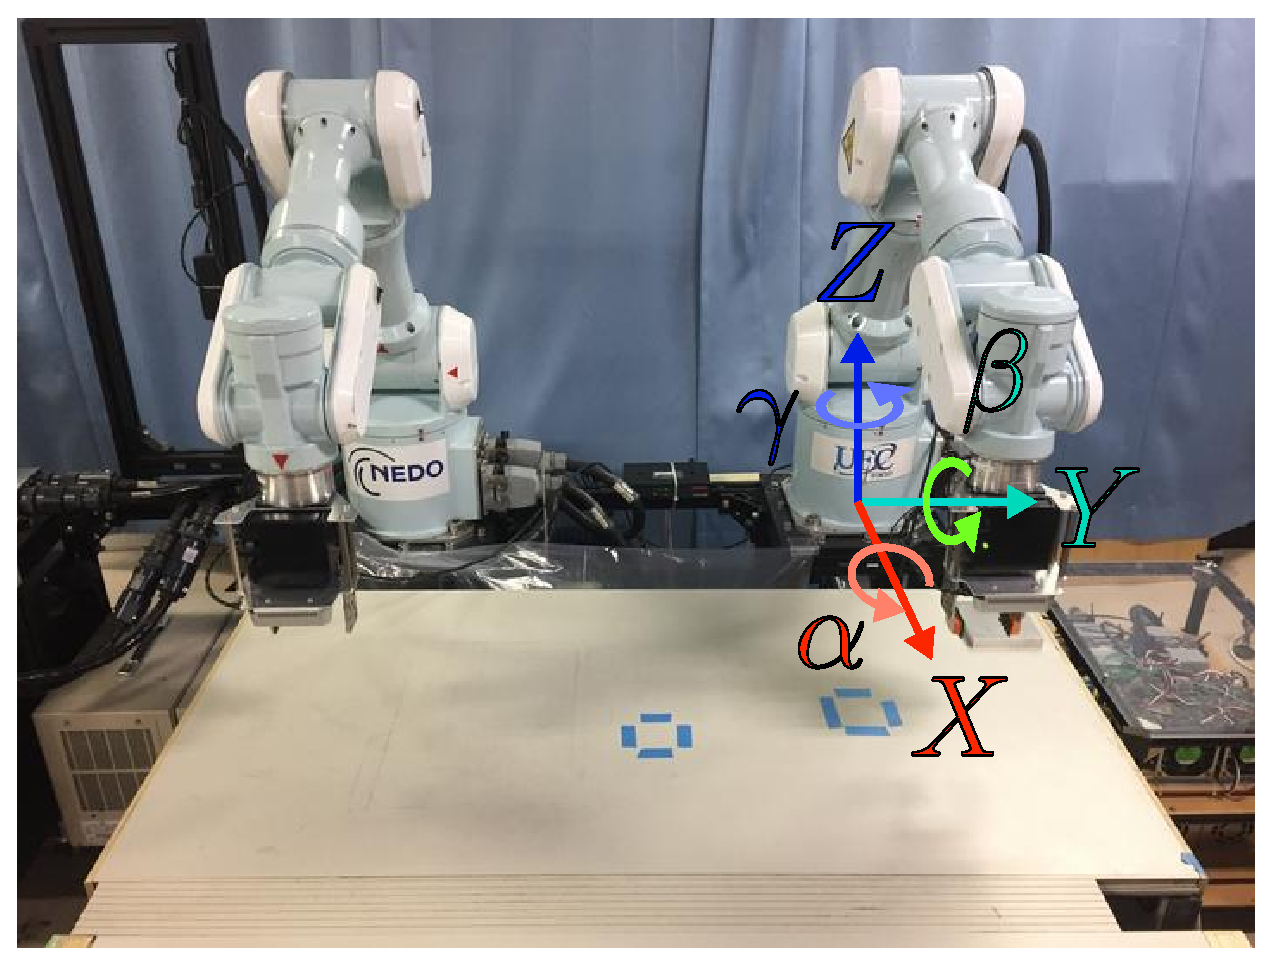
\includegraphics[width=0.7\linewidth]{fig/chp3/Coordinate_small}
		\caption{ロボットシステム}
		\label{fig:robot_system}
	\end{figure}
		
		\subsubsection{ツール座標系}
		ツール座標系はロボットが操る道具の座標系である．
		道具を目的が達成できる位置や姿勢にするとき，ロボットの手先座標系を制御するより，直接操る道具の座標系を制御する方が遥かにしやすい．
		
		PAライブラリーを用いることによってPA10の手先の位置姿勢を制御することは可能である．
		しかし，今回はツールを装着したままで実験を行い，直接ツール先端の位置姿勢を制御するため，ツール座標系を設定した．
		
		具体的には，PA10手先の位置はPA10手先の中心であり，回転はベース座標系から，$Y$軸周りで180度回転させた姿勢である．
		そして，ツール座標系はPA10手先座標系の位置はツールの中心であり，回転はPA10手先座標系から，$Y$軸で180度回転させた姿勢である．
		つまり，ツール座標系の回転はベース座標系と同じである．
		更に，各種のツールに対応するため，ツール座標系の位置姿勢はプログラムで調整できる．
		\begin{figure}[h]
			\centering
			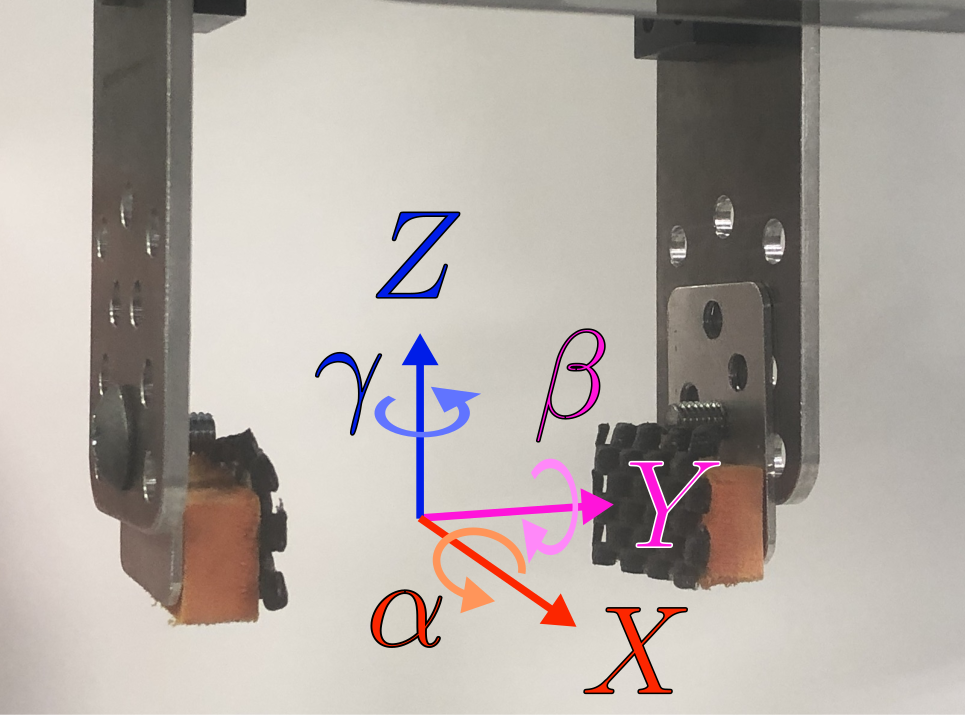
\includegraphics[width=0.7\linewidth]{fig/chp3/ToolCoordinate.png}
			\caption{ツール座標系}
			\label{fig:tool_coordinate}
		\end{figure}

	\subsection{力覚センサ}\label{sec:forcesensor}
		両腕の手首の部分に，Leptrino製の6軸力覚センサPFS080YA501U6S(図\ref{fig:robot_force})を装備し，USBでPCに接続している．
		\begin{figure}[h]
			\centering
			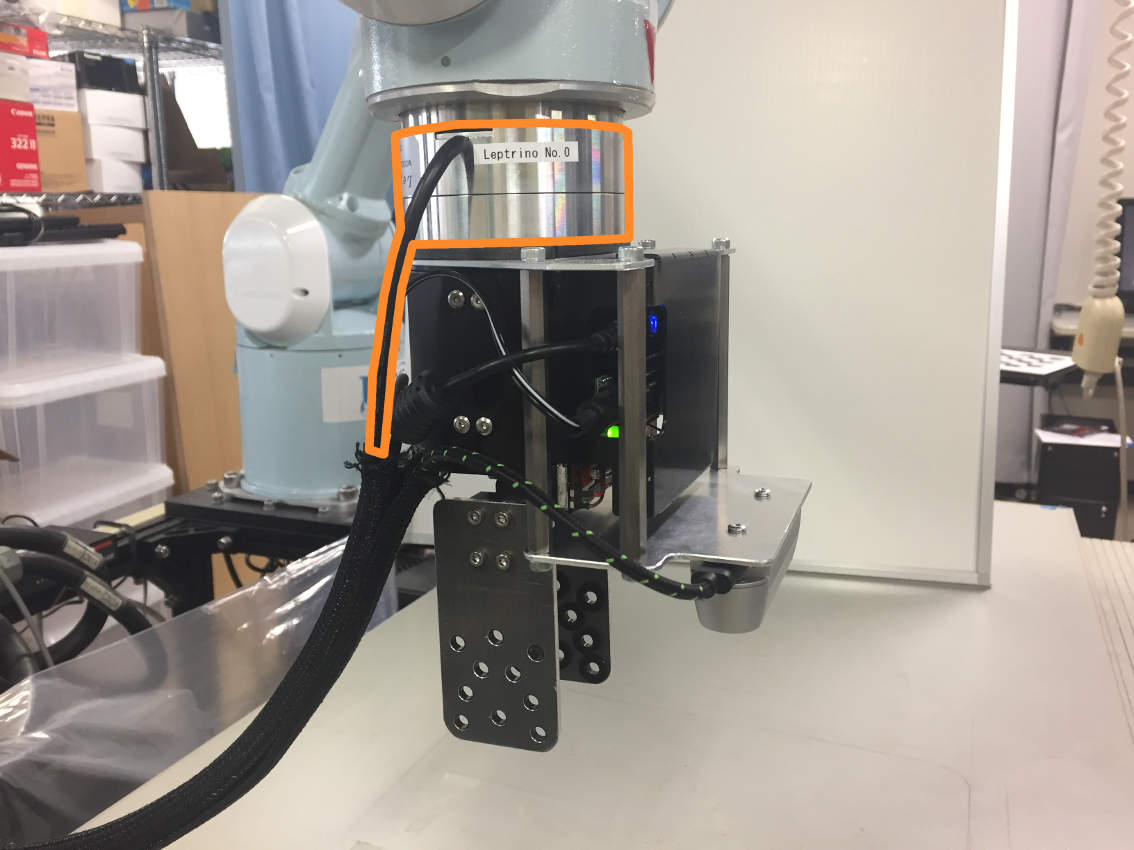
\includegraphics[width=0.7\linewidth]{fig/chp3/ForceSensor}
			\caption{力覚センサ(オレンジの枠内)}
			\label{fig:robot_force}
		\end{figure}
	
	この力覚センサの性能パラメータは(図\ref{fig:robot_force_para})
		\begin{figure}[h]
			\centering
			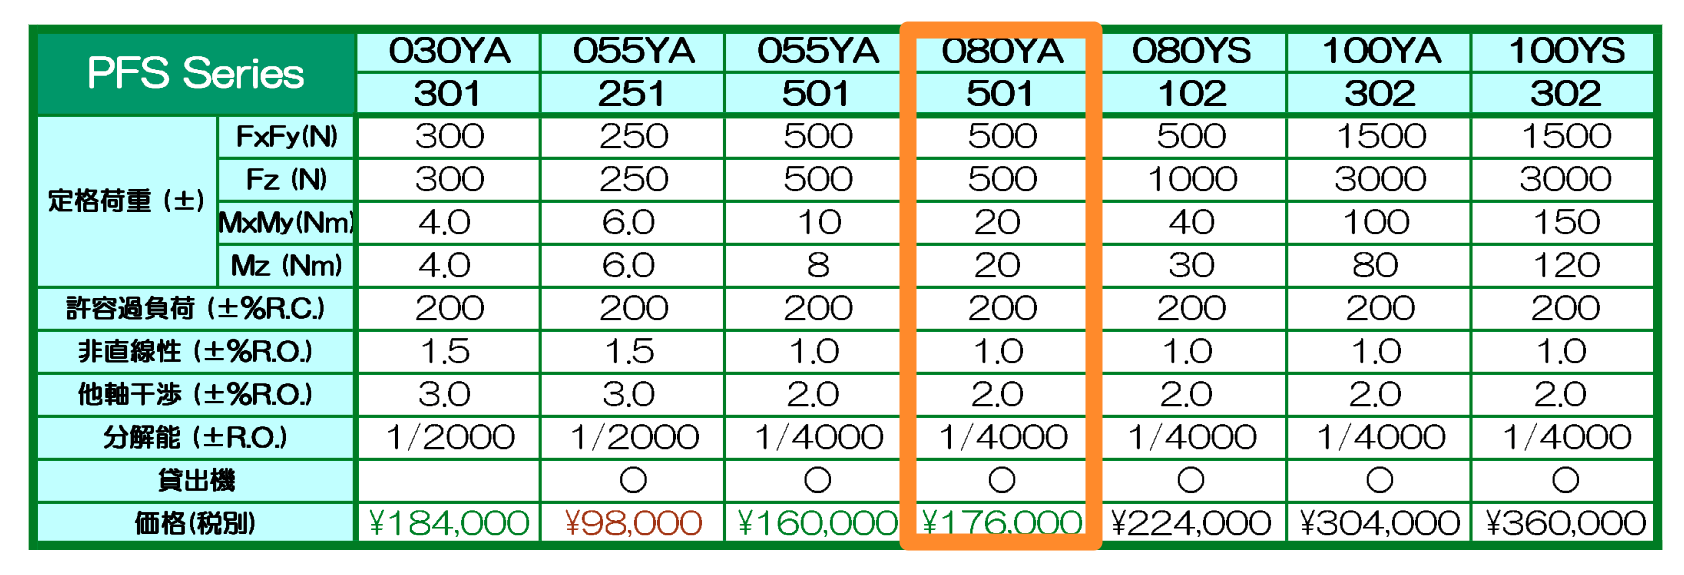
\includegraphics[width=0.7\linewidth]{fig/chp3/ForceSensor-performence}
			\caption{力覚センサのデータシート(オレンジの枠内)}
			\label{fig:robot_force_para}
		\end{figure}
	
	このデータシートにより，我々のグループで使用した力覚センサの分解能力は		
	\begin{equation}
	\begin{split}
	Resolution &= 定額荷重 \times 分解能 \\
	&= 500\mathrm{N} \times (1 / 4000)\\
	&= 0.125\mathrm{N} \\
	&= 0.125\mathrm{N} \div 9.8\mathrm{w} \\
	&\approx 0.012755\mathrm{w} \\
	&= 12.76\mathrm{w} \\
	\end{split}
	\end{equation}
	12.76gである．

	\subsection{グリッパ}
	力覚センサの下に取り付けたのは平行グリッパである．平行グリッパは1E-HM01 HANDを使い，長野らによって指先のアルミ板は様々な姿勢でツールを取り付けできるように穴が多数空いている．\cite{長野さんの修論}
	\begin{figure}[h]
		\centering
		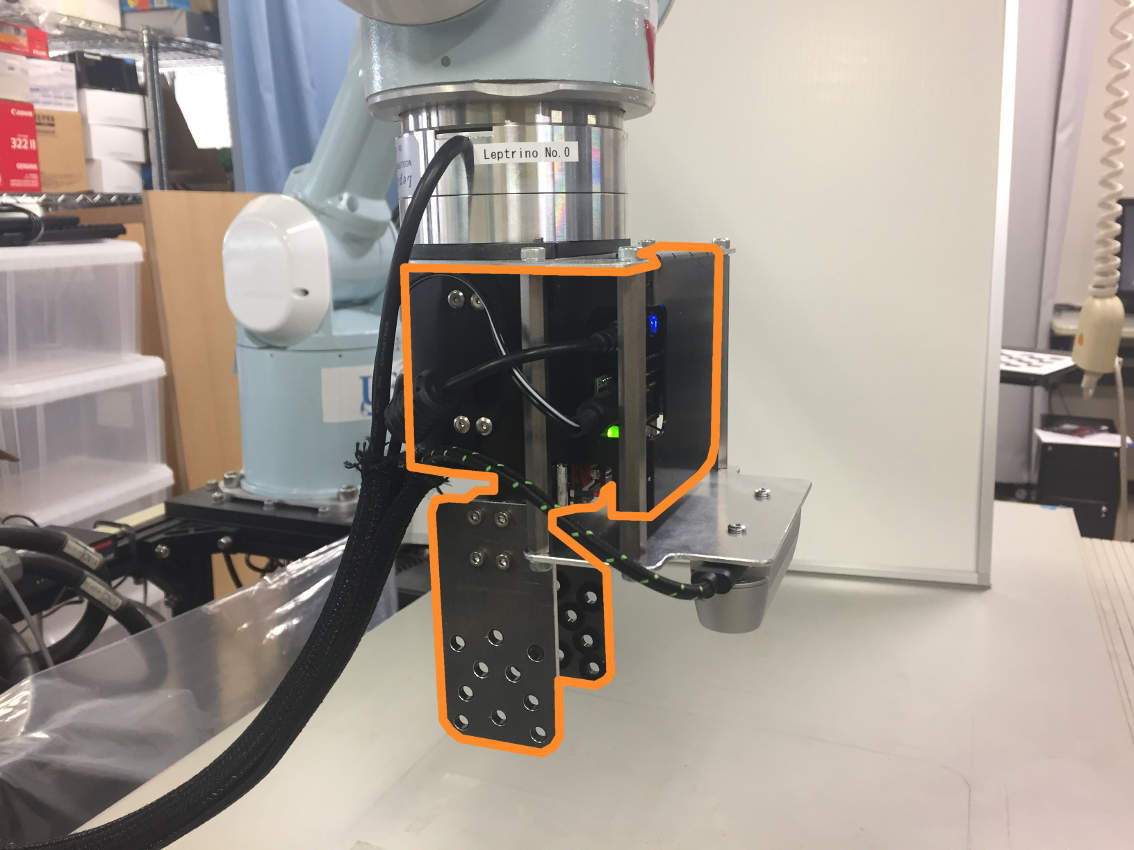
\includegraphics[width=0.7\linewidth]{fig/chp3/Gripper}
		\caption{平行グリッパ(オレンジの枠内)}
		\label{fig:robot_gripper}
	\end{figure}
	
	\subsection{エンドエフェクタ}\label{sec:endeffector}
	今回の注ぎ作業において，各種の容器を持ち上げることが必要と想定され，指先のアルミ板に2種類のエンドエフェクタを取り付けた．
		\subsubsection{その1}
		図\ref{fig:robot_gripper_1}のように，このエンドエフェクタの目的は：
		グリッパの開く距離が10[cm]しかないため，ボールやコップなどを掴むのは難しいと想定される．その場合は，容器の縁部分を掴むこととする．
		そして，摩擦力を増加させる目的でアルミ板上に小さなスポンジをつけた．
		\begin{figure}[h]
			\centering
			
\includegraphics[width=0.7\linewidth]{fig/chp3/EndFactor-1}
			\caption{エンドエフェクタ1}
			\label{fig:robot_gripper_1}
		\end{figure}
	
		\subsubsection{その2}
		図\ref{fig:robot_gripper_2}のように，このエンドエフェクタの目的は：
		10[cm]以内の容器を確実に掴むことで，摩擦力を増加させる目的でアルミ板の上に薄いスポンジをつけた．
		\begin{figure}[h]
			\centering
			
\includegraphics[width=0.7\linewidth]{fig/chp3/EndFactor-2}
			\caption{エンドエフェクタ2}
			\label{fig:robot_gripper_2}
		\end{figure}

	\subsection{視覚センサ}
	図\ref{fig:robot_camera}のように，グリッパの前面に取り付けたのは本論文に使われる視覚センサ，Intel製RealsenseD435 (RGB-Dカメラ)である．
	\begin{figure}[h]
		\centering
		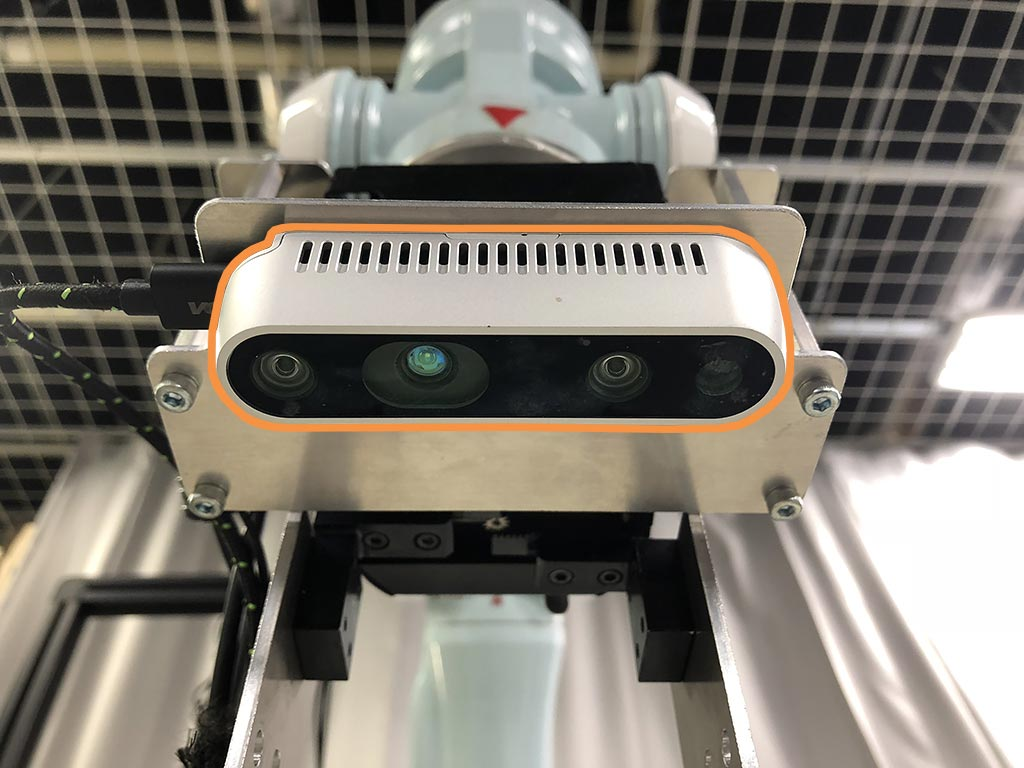
\includegraphics[width=0.7\linewidth]{fig/chp3/Realsense}
		\caption{Realsense D435}
		\label{fig:robot_camera}
	\end{figure}
	本センサは以前の視覚センサより，反射の強い材質(陶磁器や液面やトマトの表面など)に対して正確に表面のデプスデータが取れ，精度も従来より高い．
	したがって，RealsenseD435を使えば，より完全や高精度の点群データが得られる．
	今回は同時に違い角度から点群を撮る目的で，RealsenseD435を両手に取り付けた．
		
\section{ソフトウェア}
	\subsection{librealsense}
	librealsenseはIntel社がrealsenseシリーズのカメラを操作するためのクロスプラットフォームSDKである．
	使用できるプログラミング言語は，C++のほか，pythonやmatlabやLabViewなどである．
	そして，librealsenseに提供されているラッパーを利用すれば，他のライブラリーやゲームエンジン(例えば，PCLやOpenCVやUnityなど)にセンサのデータを簡単に送れる．
	
	また，このライブラリはカメラにある各種センサのデータ取得をすることができる．
	その他に，センサの生データを処理する(例えば，デプス画像とカラー画像の合成やデプス画像から点群データに変換するなど)こともできる．
	また，今librealsenseは主に2つのバージョンがある：1.Xと最新版の2.X(本論文の執筆時点で最新版は2.17．)である．
	最新版の2.Xは新しいシリーズのカメラ(D400とSR300)にのみ対応している．
	
	
	今回はRealsenseD435を使用するため，librealsenseは2.11を用いる．
	
	\subsection{PCL(Point Cloud Library)}\label{sec:pcl}
	PCL(Point Cloud Library)は2D3Dデータを処理するライブラリである．
	オープンソースのプロジェクトであり、日々更新されていてる。そのためPCLライブラリは最新の論文にあるデータ処理手法を書き込むことが可能になる．
	
	そして，機能面については，PCLライブラリは点群データを処理に必要な手法を全てモジュール化した．
	例えば，ノイズ処理のフィルターモジュール，
	点群データの特徴を抽出するフィーチャーモジュール，
	点群を合成させるregistrationモジュール，
	ある点の近傍をサーチするKD-Treeモジュール，
	点群を分割するセグメンテーションモジュール，
	点群を表示しやすくするための可視化モジュール等である．
	
	最新版は1.9.1だが，本論文は1.8.0を使う．
	
	\subsection{OpenRTM}
	本研究では RT-Middlewareの実装のひとつであるOpenRTM-aist\cite{RTM-aist}を用いてコンポーネント指向のロボット操作システムを構築した.
	以下では, RTC 毎にその詳細と全体的な接続について述べる.
		
		\subsubsection{システム全体の接続構成}
		図\ref{fig:AllConnections}に示した通り，
		前節で述べた各ハードウェアをRT-Component(RTC)として作成し,RTC-handle\cite{rtc_handle}を用いてこれらをつなぎ合わせ,全体を統括した.
		pythonのスクリプトから関数をコールすることでrtc-handleを介して各RTCに指令を送る.
		\begin{figure}[h]
			\centering
			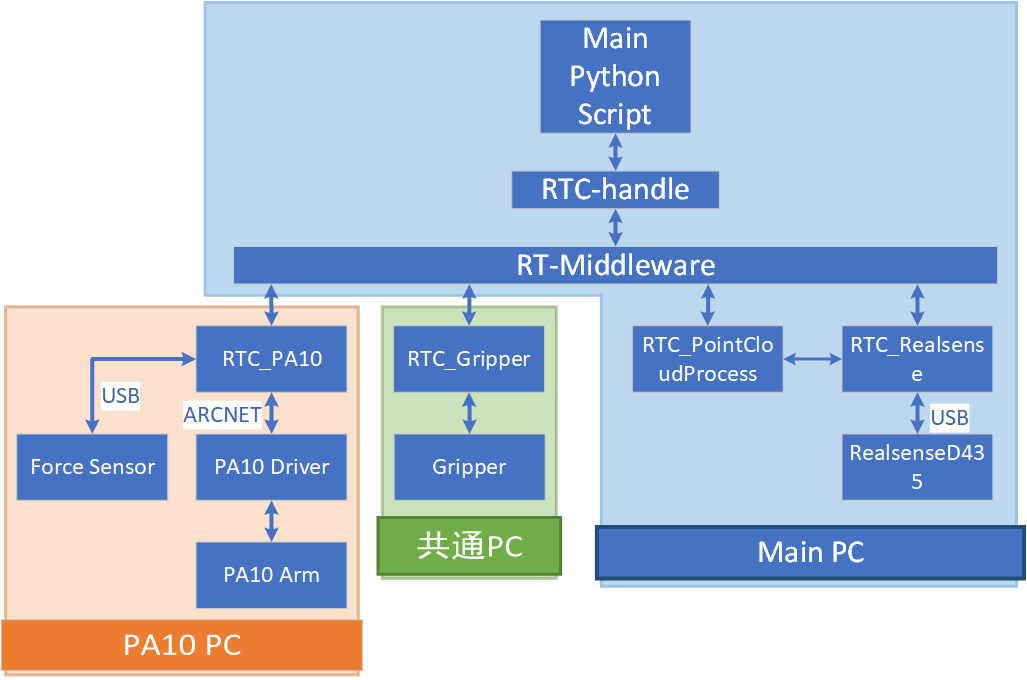
\includegraphics[width=0.9\linewidth]{fig/chp3/AllConnection.png}
			\caption{全体の接続}
			\label{fig:AllConnections}
		\end{figure}
	
		\subsubsection{RTC\_PA10}
		RTC\_PA10はPA10を操作するためのRTCである．
		このRTCは独立のPC(図\ref{fig:AllConnections}のPA10 PC)で常に実行している．
		このRTCは三菱重工が提供するPAライブラリを使っていて，ARCNETを通じてPA10のドライバと通信し，PA10を制御する．
		そして力のフィードバックでロボットの動きを制御するため，力覚センサの操作メソッドもこのRTCに組み込んだ．
		
		RTC\_PA10のインポートとアウトポートは図\ref{fig:RTCPA10}のように示す．
		\begin{figure}[h]
			\centering
			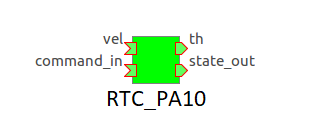
\includegraphics[width=0.5\linewidth]{fig/chp3/PA10Diag.png}
			\caption{RTC\_PA10}
			\label{fig:RTCPA10}
		\end{figure}
		
		\subsubsection{RTC\_Gripper}
		RTC\_Gripperは手先のグリッパを制御するためのRTCである．
		具体的には，グリッパの開く，閉じる動きを制御できる．
		また，メンテンナンスをしやすくするため，各手のグリッパのRTCは各PA10 PCで実行せず，共通PCで同時に実行している．
		
		最後に，RTC\_PointCloudProcessのインポートとアウトポートは図\ref{fig:RTCGripper}のように示す．
		\begin{figure}[h]
			\centering
			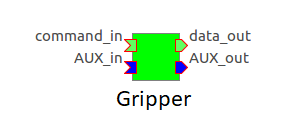
\includegraphics[width=0.5\linewidth]{fig/chp3/GripperDiag.png}
			\caption{RTC\_Gripper}
			\label{fig:RTCGripper}
		\end{figure}
		
		\subsubsection{RTC\_Realsense}
		RTC\_Realsenseは前節で紹介したlibrealsenseを使い，RealsenseD435のデータを取得し，RTC\_PointCloudProcessに送るためのRTCである．
		このRTCはカラー画像，赤外線の画像，デプス画像をRealsenseD435から読み込んで，データタイプをRTCのタイプに変換し，RTC\_PointCloudProcessに送る．
		また，前節で紹介した通り，librealsenseのデータ処理機能もRTCに書き込んだ．
		それは：
		\begin{enumerate}
			\item デプス画像から点群データへの変換プログラム．
			\item カラー赤外線の画像から点群データにマッピングするプログラム．
			\item デプス画像のノイズ処理プログラム．
		\end{enumerate}
	
		次に，上に書いたデータ処理機能とRealsenseD435からのデータの読み込みの速度を合わせるため，各データチャンネル(カラーや赤外線2つやデプス)にキューを設置した．
		これらのキューはいつも最新のデータをキューの末端に入れ続けている．
		もし，キューが満たされた時，新しいデータが来ると，新しいデータを末端に入れ，最も古いデータである先端のデータは捨てられる．
		よって，キューから読み出すデータはいつも最新のデータである．
		ここで，データの遅延を少なくするため，キューの大きさは5個に設定する．
		
		最後に，RTC\_Realsenseのインポートとアウトポートは図\ref{fig:RTCRealsense}のように示す．
		\begin{figure}[h]
			\centering
			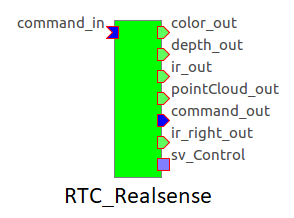
\includegraphics[width=0.5\linewidth]{fig/chp3/RealsenseDiag.png}
			\caption{RTC\_Realsense}
			\label{fig:RTCRealsense}
		\end{figure}
		
		\subsubsection{RTC\_PointCloudProcess}
		RTC\_PointCloudProcessは\ref{sec:pcl}節で紹介したPCLを使い，RTC\_Realsenseが取得した点群データを処理するRTCである．
		
		処理の基本的な流れは図\ref{fig:PCL-Process}のようになる．\par
		\begin{figure}[h]
			\centering
			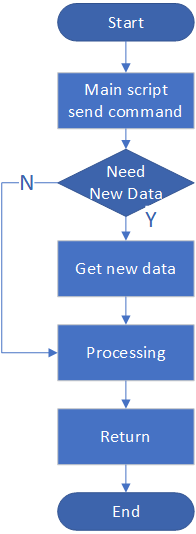
\includegraphics[width=0.35\linewidth]{fig/chp3/PCL-Process.png}
			\caption{処理の流れ}
			\label{fig:PCL-Process}
		\end{figure}
		\begin{enumerate}
			\item Pythonのメインスクリプトはサービスポートを通し，処理命令及び命令に必要なパラメータをRTC\_PointCloudProcessに送る．
			\item 命令により，RTC\_PointCloudProcessのデータポートから点群を読み出す．
			\item アルゴリズムで点群を処理する．
			\item 結果をサービスポートでメインスクリプトに返却する．
		\end{enumerate}
		つまり，2章で紹介したアルゴリズム及び4章の実装で点群を処理することに関する部分は全てこのRTCに組み込んだ．
		
		% DONG　赤い部分が修正した．
		そして，今年はRTC\_PointCloudProcessを従来の1つの受信データポートから4つのポートに増加した．
		なぜなら，同時に複数の視点から点群を撮ることや両手のどちらかが取りにくくなる場合に備えるためである．
		4つのポートにした理由は両手以外の場所(天井カメラなど)にカメラを設置することを備えるためである．
		また，今回は両手のカメラだけで，残した2つのデータポートは接続しない．

		最後に，RTC\_PointCloudProcessのインポートとアウトポー
		トは図\ref{fig:RTCPointCloudProcess}のように示す．
		\begin{figure}[h]
			\centering
			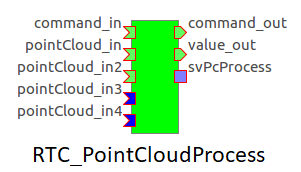
\includegraphics[width=0.5\linewidth]{fig/chp3/PointCloudProcessDiag.png}
			\caption{RTC\_PointCloudProcess}
			\label{fig:RTCPointCloudProcess}
		\end{figure}
		
		\subsubsection{RTC全体接続}
		RTC全体接続状況は図\ref{fig:SystemDiag}で示した．
		
		MainScriptはrtc-handleを実行しているメインのPythonのプログラムをRTCの模式図の形で表現したものである. 
		今回は画像のデータが使用しないため，RTC\_Realsenseのcolor\_out,depth\_out,ir\_out,ir\_right\_outデータポートの接続が表示しない．
		注ぎ作業を記述したPythonのプログラムを実行することでシステム全体を統括制御している.
		\begin{figure}[h]
			\centering
			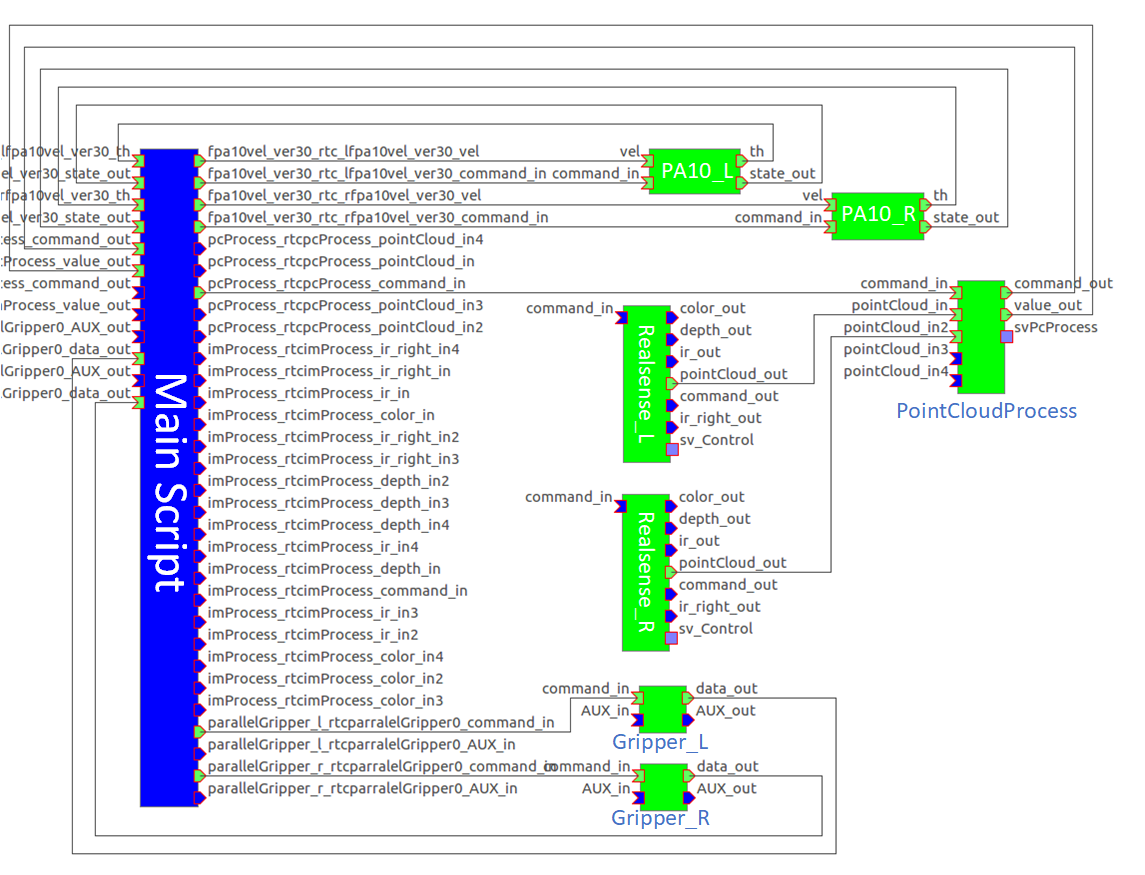
\includegraphics[width=0.9\linewidth]{fig/chp3/SystemDiag.png}
			\caption{RTC全体接続}
			\label{fig:SystemDiag}
		\end{figure}
		